% !TEX root = IBL-InsolvabilityOfQuintic.tex
\chapter{Rings}
\label{chapter:Rings}
\thispagestyle{empty}
Our overarching goal, laid out in Chapter~\ref{chapter:PolyEquations}, is to show that there are quintic polynomials whose roots are \emph{not} expressible in terms of its coefficients using just the operations of addition, subtraction, multiplication, division, and the extraction of roots (thus implying that there is no ``quintic formula'' that is analogous to the quadratic formula). We decided that we would say that such polynomials are \emph{not} solvable by radicals, and in Chapter~\ref{chapter:SolvabilityByRadicals}, we finally were able to write down a formal definition of this term. We also proved there are many polynomials that are solvable by radicals. But, how do we show that a polynomial  is \emph{not} solvable by radicals? We start by taking a closer look at polynomials.


% % % % % % % % % % % % % % % % % % % % % % % % % % % % % % % % % % % % % % % % % % % %
% % % % % % % % % % % % % % % % % % % % % % % % % % % % % % % % % % % % % % % % % % % %
% SECTION
% % % % % % % % % % % % % % % % % % % % % % % % % % % % % % % % % % % % % % % % % % % %
% % % % % % % % % % % % % % % % % % % % % % % % % % % % % % % % % % % % % % % % % % % %
\section{Abstract rings}
As we investigate polynomials, it will be useful to harness (and abstract) the algebraic properties that they possesses. For example, if we add two polynomials in $\mathbb{Q}[x]$, we obtain a polynomial that is again in $\mathbb{Q}[x]$, and similarly for multiplication. Let's explore the structure of $F[x]$ in general (where $F$ is any field). 

\begin{definition}
Let $F$ be a field. The structure $(F[x],+,\cdot)$ consists of the set $F[x]$ together with the operations $+$ and $\cdot$ defined as follows. Let $p(x) = a_0 + a_1x + \cdots + a_mx^m$ and $q(x) = b_0 + b_1x + \cdots + b_nx^n$ with $m\le n$.
\begin{itemize}
\item \textbf{Addition:} $p(x) + q(x) =  (a_0 + b_0) + (a_1 + b_1)x + \cdots + (a_n + b_n)x^n$ (where $a_k = 0$ when $k> m$).
\item \textbf{Multiplication:} $p(x)\cdot q(x) = \displaystyle\sum_{k=0}^{m+n}c_kx^k$ where $c_k = a_0b_k + a_1b_{k-1} + \cdots + a_{k-1}b_1 + a_kb_0$.
\end{itemize}
We often refer to the entire structure $(F[x],+,\cdot)$ as simply $F[x]$.
\end{definition}

In the definition of polynomial multiplication above, $p(x)\cdot q(x)$ is just the result of applying the distributive law repeatedly to $(a_0 + a_1x + \cdots + a_mx^m)\cdot(b_0 + b_1x + \cdots + b_nx^n)$ and then grouping according to the powers of $x$. We will see that the operations of polynomial addition and multiplication have many familiar properties; let's prove a couple. 

\begin{problem}
Using the definitions of polynomial addition and multiplication  together with properties of fields, prove that for all fields $F$, both addition and multiplication in $F[x]$ are commutative.
\end{problem}

\begin{problem}
Let $F$ be any field. Find an additive identity for $F[x]$, and prove that it works. Also, if $p(x) = a_0 + a_1x + \cdots + a_mx^m$ is an arbitrary polynomial in  $F[x]$, find its additive inverse, and prove that it works.
\end{problem}

\begin{problem}
Which elements of $\mathbb{Q}[x]$ have a multiplicative inverse? Which do not? Justify your answer.
\end{problem}

As should be becoming clear, many of the properties of $F$ transfer to $F[x]$ (but not all!). Let's record some of those properties in a fact, which we will not prove. The existence of multiplicative inverses is notably absent.

\begin{fact}\label{fact.PolyRingAlgProperties}Let $F$ be any field. The following are true for $F[x]$.
\begin{itemize}
\item \textbf{Addition Laws:} Addition is associative and commutative. There is a unique additive identity, namely the constant zero polynomial, and every polynomial $p(x)$ has a unique additive inverse, denoted $-p(x)$.
\item \textbf{Multiplication Laws:} Multiplication is associative and commutative. There is a unique multiplicative identity, namely the constant polynomial $1$.
\item \textbf{Distributivity Laws:} For all $p(x),q(x),r(x) \in F[x]$, $p(x)(q(x)+r(x)) = p(x)q(x)+p(x)r(x)$ and $(q(x)+r(x))p(x) = q(x)p(x)+r(x)p(x)$.
\end{itemize}
\end{fact}

% % % % % % % % % % % % % % % % % % % % % % % % % % % % % % % % % % % % % % % % % % % %
% SUBSECTION
% % % % % % % % % % % % % % % % % % % % % % % % % % % % % % % % % % % % % % % % % % % %
\subsection{Definition and first examples}

Since $F[x]$ lacks multiplicative inverses for many of its elements, it does not form a field. Nevertheless, motivated by our desire to study polynomials, we will abstract the structure that is present so that we can prove theorems about polynomials over any field, instead of  working one field at a time. However, before we do, it's worth noting that there are many other structures that are not fields but do satisfy the laws in Fact~\ref{fact.PolyRingAlgProperties}---perhaps the most prominent one is the integers $\mathbb{Z}$. We  arrive at the definition of a ring.

\begin{definition}
A \textbf{ring} is a structure $(R,+,\cdot)$ consisting of a set $R$ together with two binary operations $+$ and $\cdot$ (which we call \emph{addition} and \emph{multiplication}) such that for some element $0\in R$ the following axioms hold.
\begin{itemize}
\item \textbf{Addition Axioms:} Addition is associative and commutative; the element $0$ is an additive identity; every  $x\in R$ has an additive inverse with respect to $0$, denoted $-x$.
\item \textbf{Multiplication Axioms:} Multiplication is associative.
\item \textbf{Distributivity Axioms:} For all $x,y,z \in R$, $x(y+z) = xy+xz$ and $(y+z)x = yx+zx$.
\end{itemize}
In the case that multiplication is commutative, $R$ is called a \textbf{commutative ring}, and in the case that there is a multiplicative identity, $R$ is called a \textbf{ring with unity} (or ring with $1$). 
\end{definition}

The notion of a ring is quite general, and the  terminology  ``commutative ring'' and ``ring with unity'' highlight some of the additional properties that $F[x]$ has, but arbitrary rings may not. But notice that fields have all of these properties \emph{and more}. The next definition  is meant to highlight this.

\begin{definition}
A \textbf{division ring} is a ring with unity such that every nonzero element has a multiplicative inverse.
\end{definition}

\begin{problem}
Fill in each box of the table below with \textbf{Y}es or \textbf{N}o. Assume that  $+$ and $\cdot$ are defined ``as usual'' for each set.\footnote{$2\mathbb{Z}$ denotes the even integers. The operations are usual integer addition and multiplication.}
\begin{flushleft}
\tabulinesep = 2mm
\begin{tabu}  {X[1.25,c,m]|[2pt]X[.8,c,m]|X[c,m]|X[c,m]|X[c,m]|X[.8,c,m]}
 & ring & commutative ring & ring with unity & division ring & field \\ \tabucline[2pt]{-}
$\mathbb{Z}$ &&&&& \\  \hline 
$2\mathbb{Z}$  &&&&& \\ \hline 
$\mathbb{N}$ &&&&& \\ \hline 
$\mathbb{Q}$ &&&&& \\ \hline 
$\mathbb{H}$ &&&&& \\ \hline 
$\mathbb{Z}_6$ &&&&& \\ \hline 
$\mathbb{R}[x]$ &&&&& \\ \hline 
$\left\{ a + bi\mid a,b\in \mathbb{Q}\right\}$ &&&&& \\ \hline 
$\left\{ a + bi\mid a,b\in \mathbb{Z}\right\}$ &&&&& \\ \hline 
\end{tabu}
\end{flushleft}
\end{problem}

% % % % % % % % % % % % % % % % % % % % % % % % % % % % % % % % % % % % % % % % % % % %
% SUBSECTION
% % % % % % % % % % % % % % % % % % % % % % % % % % % % % % % % % % % % % % % % % % % %
\subsection{Basic properties}

Many of the basic properties of fields hold also for rings, with essentially the same proofs, so we will just take them as fact.

\begin{fact}[Compare with Fact~\ref{thm.BasicFieldPropsUniqueness}]
Let $R$ be a ring. 
\begin{enumerate}
\item The additive identity is unique. If there exists a multiplicative identity, it is  unique.
\item Additive inverses are unique. If an element has a multiplicative inverse, it is unique.
\end{enumerate}
\end{fact}

\begin{fact}[Compare with Fact~\ref{thm.BasicFieldProps}]
Let $R$ be a ring. 
\begin{enumerate}
\item For all $x\in R$, $x\cdot0 = 0 = 0\cdot x$.
\item For all $x,y\in R$, $(-x)y = -(xy)$ and $x(-y) = -(xy)$.
\item If $R$ contains at least two elements and has a multiplicative identity, then the additive and multiplicative identities are different, i.e.~$0\neq 1$.
\end{enumerate}
\end{fact}

Let's explore one further property that fields possess but is not listed above: for all $x$ and $y$ in a field, if $xy = 0$, then $x=0$ or $y=0$. 

\begin{definition}
Let $R$ be a ring. An element $a\in R$ is called a \textbf{zero divisor} if $a$ is nonzero and there exists a nonzero $b\in R$ such that $ab=0$. A ring is called an  \textbf{integral domain} if it is a commutative ring with unity containing at least two elements but \emph{no zero divisors}.
\end{definition}

As remarked above, fields do not have zero divisors, so every field is indeed an integral domain. However, the prototypical integral domain (which explains the choice of name) is $\mathbb{Z}$. Let's look for others.

\begin{problem}
For each of the following rings, determine if there are zero divisors, and if so, find them all. Is the ring an integral domain?
\begin{multicols}{2}
\begin{enumerate}
\item $\mathbb{Z}_{5}$
\item $\mathbb{Z}_{10}$
\item $\mathbb{H}$
\item $\mathbb{R}[x]$
\end{enumerate}
\end{multicols}
\end{problem}

When working with integral domains, the following property is key.

\begin{theorem}[Cancellation Property]\label{thm.IntegralDomainCancel}
Let $R$ be an integral domain. For all $a,b,c\in R$, if $ab = ac$, then either $a=0$ or $b=c$. 
\end{theorem}

\begin{problem}
What properties of integral domains did you use in your proof of Theorem~\ref{thm.IntegralDomainCancel}? Can you rewrite the theorem to be more general? Try.  
\end{problem}

Let's pause to collect and organize all of our new definitions.

\begin{problem}
Complete the following Venn Diagram by adding in shapes for each of the following terms. Try to provide examples that live in each of the gaps, but we have not encountered enough examples (in these notes) to cover all gaps yet.
\begin{multicols}{3}
\begin{itemize}
\item Fields
\item Rings
\item Commutative Rings
\item Rings with unity
\item Division Rings
\item Integral domains
\end{itemize}
\end{multicols}
\begin{center}
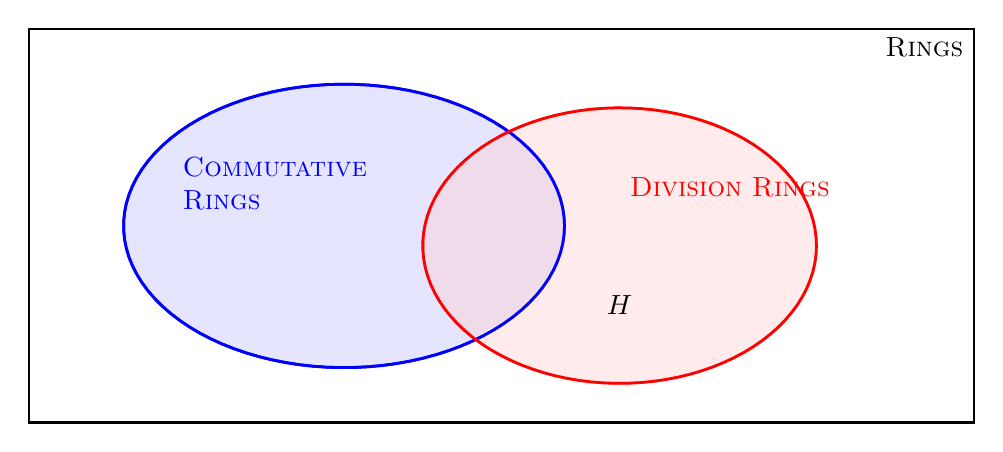
\begin{tikzpicture}[line width = 1]
\draw (0,0) rectangle (12,5);
\begin{scope}[shift={(4,2.5)}]
\fill[domain = 0:360,draw = blue, fill = blue!10, samples = 100] plot ({2.8*cos(\x)},{1.8*sin(\x)});
\end{scope}
\begin{scope}[shift={(7.5,2.25)}]
\fill[domain = 0:360,draw = red,fill = red!20, samples = 100,opacity=0.4] plot ({2.5*cos(\x)},{1.75*sin(\x)});
\end{scope}
\begin{scope}[shift={(4,2.5)}]
\draw[domain = 0:360,draw = blue, samples = 100,] plot ({2.8*cos(\x)},{1.8*sin(\x)});
\end{scope}
\begin{scope}[shift={(7.5,2.25)}]
\draw[domain = 0:360,draw = red, samples = 100] plot ({2.5*cos(\x)},{1.75*sin(\x)});
\end{scope}
\node[black, anchor = 20] at (12,5) {\textsc{Rings}};
\node[blue, anchor = 20, text width = 1in, align = flush left] at (4.5,3.5) {\textsc{Commutative Rings}};
\node[red, anchor = 20, text width = 1in, align = flush right] at (9.6,3.25) {\textsc{Division Rings}};
\node at (7.5,1.5) {$\mathbb{H}$};
\end{tikzpicture}
\end{center}
\end{problem}

% % % % % % % % % % % % % % % % % % % % % % % % % % % % % % % % % % % % % % % % % % % %
% SUBSECTION
% % % % % % % % % % % % % % % % % % % % % % % % % % % % % % % % % % % % % % % % % % % %
\subsection{Units}

Unless $R$ is actually a division ring, not all elements of $R$ will have a multiplicative inverse. Let's explore those elements that \emph{do} have an inverse.

\begin{definition}
Let $R$ be a ring with unity containing at least two elements. Then, $u\in R$ is called a \textbf{unit} if $u$ has a multiplicative inverse. The set of all units in $R$ is denoted $U(R)$.
\end{definition}


\begin{problem}
For each of the following rings, find all of the units, i.e.~determine $U(R)$.
\begin{multicols}{2}
\begin{enumerate}
\item $\mathbb{Z}$
\item $\mathbb{Z}_{5}$
\item $\mathbb{R}$
\item $\mathbb{R}[x]$
\end{enumerate}
\end{multicols}
\end{problem}

\begin{problem}
Consider the ring $\mathbb{Z}_{20}$. Find all units of $\mathbb{Z}_{20}$ and also find all zero divisors. What do you notice?
\end{problem}

\begin{problem}
Let $n$ be a positive integer. Make a conjecture about $U(\mathbb{Z}_n)$ by filling in the blank:  $U(\mathbb{Z}_n) = \{a\in \mathbb{Z}_n\mid\text{ \fillInBlank{fill in the blank} }\}$. What evidence do you have?
\end{problem}

\begin{theorem}\label{thm.UnitIsNotZeroDivisor}
Let $R$ be a ring with unity containing at least two elements. If $u\in R$ is a unit, then $u$ is \emph{not} a zero divisor.
\end{theorem}

\begin{problem}
Either prove or disprove the \emph{converse} of Theorem~\ref{thm.UnitIsNotZeroDivisor}.
\end{problem}

\begin{theorem}\label{thm.UnitsFormGroup}
Let $R$ be a ring with unity containing at least two elements. Then $(U(R),\cdot)$ is a group.
\end{theorem}


% % % % % % % % % % % % % % % % % % % % % % % % % % % % % % % % % % % % % % % % % % % %
% % % % % % % % % % % % % % % % % % % % % % % % % % % % % % % % % % % % % % % % % % % %
% SECTION
% % % % % % % % % % % % % % % % % % % % % % % % % % % % % % % % % % % % % % % % % % % %
% % % % % % % % % % % % % % % % % % % % % % % % % % % % % % % % % % % % % % % % % % % %
\section{An aside: matrix rings}

Matrix rings are really the prototypical ring with unity. Although you may have only seen matrices with real entries, it turns out that we can do matrix arithmetic with other types of entries, e.g.~entries from $\mathbb{C}$ or $\mathbb{Z}$. In fact, the usual matrix addition and multiplication makes sense when the entries come from any ring.

\begin{definition}
Let $R$ be a ring and $n$ a positive integer. Then $M_{n}(R)$ denotes the set of all $n\times n$ matrices whose entries come from $R$. The structure $(M_{n}(R),+,\cdot)$ consists of the set $M_{n}(R)$ of all $n\times n$ matrices whose entries come from $R$, together with the operations of usual matrix addition and matrix multiplication. 
\end{definition}

\begin{problem}
Provide examples of matrices satisfying each of the following conditions.
\begin{multicols}{2}
\begin{enumerate}
\item $A\in M_{3}(\mathbb{C})$ but $A\notin M_{3}(\mathbb{R})$
\item $B\in M_{2}(\mathbb{H})$ but $B\notin M_{2}(\mathbb{C})$
\item $C\in M_{2}\left(\mathbb{Q}\left(\sqrt{5}\right)\right)$ but $C\notin M_{2}(\mathbb{Q})$
\item $D\in M_{2}\left(\mathbb{R}[x]\right)$ but $D\notin M_{2}(\mathbb{R})$
\end{enumerate}
\end{multicols}
\end{problem}

\begin{problem}
Verify that $M_{2}(\mathbb{Z})$ is closed under matrix multiplication.
\end{problem}

The next fact shows that $M_{n}(R)$ is a ring with unity (for each positive $n$). Afterward, we will explore some of the other ring properties we discussed above.

\begin{fact} Let $R$ be any ring. The following are true for $M_{n}(R)$.
\begin{itemize}
\item \textbf{Addition Laws:} Addition is associative and commutative. There is a unique additive identity, namely the matrix with all entries equal to $0$, and every matrix $A$ has a unique additive inverse, denoted $-A$.
\item \textbf{Multiplication Laws:} Multiplication is associative. There is a unique multiplicative identity, namely the matrix with $1$'s on the main diagonal and $0$'s everywhere else.
\item \textbf{Distributivity Laws:} For all $A,B,C \in M_{n}(R)$, $A(B+C) = AB+AC$ and $(B+C)A = BA + CA$.
\end{itemize}
\end{fact}

\begin{problem}
Is $M_{2}(\mathbb{R})$ commutative? Prove your answer.
\end{problem}

\begin{problem}
Does $M_{2}(\mathbb{R})$ have zero divisors? Prove your answer. 
\end{problem}

The collection of units in a matrix ring forms a group with respect to matrix multiplication by Theorem~\ref{thm.UnitsFormGroup}. It is a very important object and even has a special name.

\begin{definition}
Let $R$ be a ring and $n$ a positive integer. The \textbf{general linear group} over the ring $R$,  denoted $\operatorname{GL}_n(R)$, is the group of units in the ring $M_{n}(R)$.
\end{definition}

\begin{problem}
Show that $\begin{bmatrix} i & 3\\ 0& i\end{bmatrix}\in\operatorname{GL}_{2}(\mathbb{C})$ by finding a multiplicative inverse for it. Also, find two different matrices in $M_{2}(\mathbb{C})$ that are \emph{not} in  $\operatorname{GL}_{2}(\mathbb{C})$.
\end{problem}


% % % % % % % % % % % % % % % % % % % % % % % % % % % % % % % % % % % % % % % % % % % %
% % % % % % % % % % % % % % % % % % % % % % % % % % % % % % % % % % % % % % % % % % % %
% SECTION
% % % % % % % % % % % % % % % % % % % % % % % % % % % % % % % % % % % % % % % % % % % %
% % % % % % % % % % % % % % % % % % % % % % % % % % % % % % % % % % % % % % % % % % % %
\section{Polynomial rings}
Our study of rings was motivated by our desire to learn more about polynomials, and we now dive a little deeper into the theory of polynomial rings. Ultimately, we will focus on polynomials rings $F[x]$ where $F$ is a field. In this section, we will see that $F[x]$ behaves in many ways like the integers $\mathbb{Z}$: $F[x]$ is an integral domain, there is a division algorithm for $F[x]$, there exists a greatest common divisor for polynomials, and there is a notion of primes and prime factorizations. 
Let's start with some important terminology.

\begin{definition}
Let $R$ be a ring, and let  $p(x)\in R[x]$ be a \emph{nonzero} polynomial. If $p(x) = a_0 + a_1x + \cdots + a_nx^n$ with $a_n \neq 0$, then $n$ is called the \textbf{degree} of $p(x)$, denoted $\deg p(x)$. In words, $\deg p(x)$ is the highest power of $x$ in $p(x)$ with a nonzero coefficient. The degree of the zero polynomial is undefined.
\end{definition}

\begin{problem}
Determine the degree of each of the following polynomials.
\begin{enumerate}
\item $q(x) = 4x^5 + 2x^2 + 5 -8x^2 +2x^5$ in the ring $\mathbb{Z}[x]$
\item $r(x) = 4x^5 + 2x^2 + 5 -14x^2 +2x^5$ in the ring $\mathbb{Z}_6[x]$
\item $p(t) = (3t^2-\sqrt{2})(-1 + 2t -t^3)$ in the ring $\mathbb{R}[t]$
\item $s(x) = (5-i)^8 - (5-s)^8$ in the ring $\mathbb{C}[s]$
\end{enumerate}
\end{problem}

The degree function is incredibly useful when working with polynomials---let's prove a couple of properties about it. 

\begin{theorem}\label{thm.DegreePolySum}
Let $R$ be a ring. If $p(x)$ and $q(x)$ are nonzero polynomials $R[x]$, then $\deg(p(x) + q(x)) \le \max(\deg p(x),\deg q(x))$ or  $\deg(p(x) + q(x))$ is undefined.
\end{theorem}

\begin{problem}
Give an example of polynomials $p(x),q(x)\in \mathbb{Q}[x]$ such that $\deg(p(x)+q(x)) < \max(\deg p(x),\deg q(x))$.
\end{problem}

\begin{theorem}\label{thm.DegreePolyProduct}
Let $D$ be an integral domain. If $p(x)$ and $q(x)$ are nonzero polynomials $D[x]$, then $\deg(p(x)q(x)) = \deg p(x) + \deg q(x)$, and in particular, $\deg(p(x)q(x))$ is defined.
\end{theorem}

\begin{problem}
Give an example of nonzero polynomials $p(x),q(x)\in \mathbb{Z}_{10}[x]$ such that $\deg(p(x)q(x)) \neq \deg p(x) + \deg q(x)$. Why does this not contradict Theorem~\ref{thm.DegreePolyProduct}?
\end{problem}

\begin{corollary}\label{cor.PolysOverIntegralDomains}
If $D$ is an integral domain, then $D[x]$ is an integral domain.
\end{corollary}

% % % % % % % % % % % % % % % % % % % % % % % % % % % % % % % % % % % % % % % % % % % %
% SUBSECTION
% % % % % % % % % % % % % % % % % % % % % % % % % % % % % % % % % % % % % % % % % % % %
\subsection{Division algorithm}
Here we explore what it means for one polynomial to divide another as well as the idea of a quotient and remainder for division. These should be familiar from previous classes for $\mathbb{R}[x]$, but here we see that they generalize to arbitrary $F[x]$ for $F$ a field.
 
\begin{definition}
Let $R$ be a ring, and let $a,b\in R$. We say that $b$ \textbf{divides} $a$ (or $b$ is a \textbf{divisor} of $a$) if there exists some $q\in R$ such that $a = bq$.
\end{definition}

\begin{problem}
Consider the polynomial $p(x) = x^2 - 1$ in $\mathbb{Q}[x]$.
\begin{enumerate}
\item Does $x+1$ divide $p(x)$ in $\mathbb{Q}[x]$? Why or why not?
\item Does $p(x)$ divide $x+1$ in $\mathbb{Q}[x]$? Why or why not?
\item Does $3$ divide $p(x)$ in $\mathbb{Q}[x]$? Why or why not?
\end{enumerate}
\end{problem}

\begin{theorem}\label{thm.LinearFactorOfPolyImpliesRoot}
Let $p(x)\in R[x]$ with $R$ a ring. If $c\in R$ and $(x-c)$ divides $p(x)$, then $p(c) = 0$.
\end{theorem}

Even if $b(x)$ does not divide $a(x)$, it can still be useful to perform the division to obtain a quotient and remainder.

\begin{problem}
Consider the polynomials $a(x) = x^4+x^3-8x +5$  and $b(x) = x^2 -3$ in $\mathbb{Q}[x]$. Use polynomial long division to show that $b(x)$ does not divide $a(x)$. What is the quotient and what is the remainder? Write $a(x)$ as $a(x) = b(x)q(x) + r(x)$ for some $q(x),r(x)\in \mathbb{Q}[x]$ with $\deg r(x) < \deg b(x)$.
\end{problem}

The ``division algorithm'' (Theorem~\ref{thm.DivisionAlgorithm}) formalizes what results from long division. And, it turns out that it is true for polynomials over any field (not just $\mathbb{Q}$). The next lemma prepares for the proof of the division algorithm. 

\begin{lemma}
Let $F$ be a field, and let $a(x),b(x)\in F[x]$ with $\deg a(x)\ge \deg b(x)$. Assume that $a(x) = a_0 + a_1x + \cdots + a_nx^n$ with $a_n\neq 0$ and $b(x) = b_0 + b_1x + \cdots + b_mx^m$ with $b_m\neq 0$. Set $a_1(x) =  a(x) - b(x)a_nb_m^{-1}x^{n-m}$. Then $\deg a_1(x) < \deg a(x)$, and $b(x)$ divides $a(x) - a_1(x)$.
\end{lemma}

Suppose we are trying to divide $b(x)$ into $a(x)$. How do we find the quotient and the remainder? Well, if the degree of $a(x)$ is smaller than the degree of $b(x)$ there is nothing to do (and if $a(x) = 0$, there is also nothing to do). Otherwise, we can use the previous lemma to produce a polynomial $a_1(x)$ such that $\deg a_1(x) < \deg a(x)$ and $b(x)$ divides $a(x) - a_1(x)$, or in other words, $a(x) - a_1(x) = b(x)q_1(x)$ for some $q_1(x)$. Now, suppose we repeat the process and divide $b(x)$ into the resulting $a_1(x)$ to produce $a_2(x)$ and $q_2(x)$. Continuing in this fashion, we produce $a_2, q_2, a_3,q_3 \ldots, a_k,q_k$, stopping once the degree of $a_k(x)$ becomes smaller than the degree of $b(x)$ (or $a_k(x)=0$). In total, we get something like the following.

\begin{align*}
a(x) - a_1(x) & = b(x)q_1(x)\\
a_1(x) - a_2(x) & = b(x)q_2(x)\\
a_2(x) - a_3(x) & = b(x)q_3(x)\\
& \;\;\vdots\\ 
a_{k-1}(x) - a_{k}(x) & = b(x)q_k(x)
\end{align*}
Adding the above equations together and moving things around, we arrive at  \[a(x) = b(x)\left(q_1(x) + q_2(x) + q_3(x) +\cdots + q_k(x)\right) + a_k(x)\]
with the degree of $a_k(x)$ being less than the degree of $b(x)$. Thus, $a_k(x)$  is the remainder and $q_1(x) +\cdots + q_k(x)$ the quotient. This is the rough idea behind the division algorithm.

\begin{theorem}[Division algorithm for {$F[x]$}]\label{thm.DivisionAlgorithm}
Let $F$ be a field, and let $a(x),b(x)\in F[x]$ with $b(x) \neq 0$. Then there exist $q(x),r(x)\in F[x]$ such that 
\[a(x) = b(x)q(x) + r(x)\]
with $\deg r(x) < \deg b(x)$ or $r(x) = 0$.
\end{theorem}

The division algorithm is the theoretical analogue of long division. If you want to divide concrete polynomials, use long division, but if you want to prove something about divisibility for arbitrary polynomials, use the division algorithm. It is often used to prove a polynomial $b(x)$ actually divides another polynomial $a(x)$. The strategy is to apply the division algorithm to produce the equation $a(x) = b(x)q(x) + r(x)$ (with $\deg r(x) < \deg b(x)$ or $r(x) = 0$) and then use this to show that, in fact, $r(x)=0$,  implying that $a(x) = b(x)q(x)$ as desired. Let's try using this approach to prove the converse of Theorem~\ref{thm.LinearFactorOfPolyImpliesRoot}.

\begin{theorem}\label{thm.RootImpliesLinearFactorOfPoly}
Let $p(x)\in F[x]$ for $F$ a field. If $c\in F$ and $p(c) = 0$, then $(x-c)$ divides $p(x)$.
\end{theorem}

\begin{problem}
Consider the polynomial  $p(x) = x^2+x+3$ in $\mathbb{Z}_5[x]$. Compute $p(c)$ for each $c\in \mathbb{Z}_5$, and use the results to determine which polynomials of the form $(x-c)$ divide $p(x)$. Factor $p(x)$ into a product of degree $1$ polynomials in $\mathbb{Z}_5[x]$, if possible.
\end{problem}

\begin{problem}
Consider the polynomial  $p(x) = x^2+x+1$ in $\mathbb{Z}_5[x]$. Explain why $p(x)$ cannot be factored into a product of degree $1$ polynomials in $\mathbb{Z}_5[x]$.
\end{problem}

% % % % % % % % % % % % % % % % % % % % % % % % % % % % % % % % % % % % % % % % % % % %
% SUBSECTION
% % % % % % % % % % % % % % % % % % % % % % % % % % % % % % % % % % % % % % % % % % % %
\subsection{Greatest common divisors}

The fact that there is a division algorithm for $F[x]$ (Theorem~\ref{thm.DivisionAlgorithm}) is a rather special property for a ring to possess, and it has several important consequences. The first one we'll explore is the existence of a ``greatest common divisor'' for two polynomials, and our first order of business is to try to decide on a reasonable definition of this.
 
\begin{problem}
What are the common divisors of $6$ and $-9$ in $\mathbb{Z}$? Which one is the greatest common divisor?
\end{problem}

\begin{problem}\label{prob.GCDExlore}
Consider the polynomials $a(x) = 2x^2-2$ and $b(x) = 2x^2+2x-4$ in $\mathbb{Q}[x]$.
\begin{enumerate}
\item Show that $x-1$ is a common divisor of $a(x)$ and $b(x)$ by finding  $q(x),s(x)\in \mathbb{Q}[x]$ such that $a(x) = (x-1)q(x)$ and $b(x) = (x-1)s(x)$.
\item Show that $-2(x-1)$ is a common divisor of $a(x)$ and $b(x)$ by finding  $q(x),s(x)\in \mathbb{Q}[x]$  such that $a(x) = -2(x-1)q(x)$ and $b(x) = -2(x-1)s(x)$.
\item Show that $100(x-1)$ is a common divisor of $a(x)$ and $b(x)$ by finding  $q(x),s(x)\in \mathbb{Q}[x]$ such that $a(x) = 100(x-1)q(x)$ and $b(x) = 100(x-1)s(x)$.
\end{enumerate}
Which one, if any, would be a good choice as the ``greatest common divisor''?
\end{problem}

The previous problem highlights that there are several (actually, infinitely many) choices for the ``greatest common divisor'' of two polynomials. Our choice for which one we call the greatest common divisor is, in some sense, the simplest one.

\begin{definition}
A polynomial $p(x)$ of degree $n$ is called \textbf{monic} if the coefficient of $x^n$ (i.e.~the leading coefficient) is $1$.
\end{definition}

For example, $7-2x+x^2$ is monic, since the coefficient of $x^2$ is $1$. However, neither $7-2x+3x^2$ nor $7-2x-x^2$ are monic.

\begin{definition}
Let $F$ be a field, and let $a(x), b(x)\in F[x]$ be nonzero polynomials. A polynomial $d(x)\in F[x]$ is called a \textbf{greatest common divisor} of $a(x)$ and $b(x)$ if
\begin{enumerate}
\item $d(x)$ is monic,
\item $d(x)$ divides both $a(x)$ and $b(x)$,
\item if $h(x)$ divides both $a(x)$ and $b(x)$, then $h(x)$ divides $d(x)$.
\end{enumerate}
\end{definition}

Thus, in Problem~\ref{prob.GCDExlore},  the greatest common divisor of the polynomials $a(x)$ and $b(x)$ is $x-1$.
That said, we don't yet know that a greatest common divisor always exists, but let's start by showing that if one exists, there is only one.

\begin{lemma}\label{lem.GCDUnique}
Let $F$ be a field, and let $a(x), b(x)\in F[x]$ be nonzero polynomials. If $d_1(x)$ and $d_2(x)$ are  greatest common divisors of $a(x)$ and $b(x)$, then $d_1(x)=d_2(x)$.
\end{lemma}

We now work towards the existence of a greatest common divisor for arbitrary polynomials in $F[x]$ (for arbitrary fields). The proof of this result is tightly tied to analyzing certain combinations of the polynomials $a(x)$ and $b(x)$. Let's explore this a bit.

\begin{problem}\label{prob.GCDIdeal}
Consider the polynomials $a(x) = 2x^2-2$ and $b(x) = 2x^2+2x-4$ in $\mathbb{Q}[x]$.  Define \[I = \{f(x)a(x) + g(x)b(x)\mid f(x),g(x)\in \mathbb{Q}[x]\}.\]
\begin{enumerate}
\item Write down 5 different polynomials that are in the set $I$. 
\item Show that $x-1$ divides an arbitrary polynomial in $I$.
\end{enumerate}
\end{problem}

The idea behind the second part of Problem~\ref{prob.GCDIdeal} can be used to prove the following general result about sets like $I$.

\begin{theorem}\label{thm.HalfOfGCDProof}
Let $F$ be a field, and let $a(x), b(x)\in F[x]$ be nonzero polynomials. Define \[I = \{f(x)a(x) + g(x)b(x)\mid f(x),g(x)\in F[x]\}.\]
If $h(x)$ divides both $a(x)$ and $b(x)$, then $h(x)$ divides every $c(x)\in I$.
\end{theorem}

The existence and uniqueness of greatest common divisors in $F[x]$ is presented in the following fact.

\begin{fact}\label{fact.GCD}
Let $F$ be a field, and let $a(x), b(x)\in F[x]$ be nonzero polynomials. There exists a unique greatest common divisor of $a(x)$ and $b(x)$, and if $d(x)$ is the greatest common divisor, then \[d(x) = f(x)a(x) + g(x)b(x),\]
for some $f(x),g(x)\in F[x]$.
\end{fact}

The proof of this fact is interesting, but let's content ourselves to just outline it. The approach is fairly straight forward. Define \[I = \{f(x)a(x) + g(x)b(x)\mid f(x),g(x)\in F[x]\}.\]  Theorem~\ref{thm.HalfOfGCDProof} tells us that every common divisor of $a(x)$ and $b(x)$ is a divisor of every polynomial in $I$. Thus, if $I$ contains a monic, common divisor of $a(x)$ and $b(x)$, it must be the greatest common divisor. So, we look for a common divisor of $a(x)$ and $b(x)$ in $I$. And to do this, the key idea is to choose a polynomial of smallest degree in $I$.

Let $m$ be the smallest degree of all nonzero polynomials in $I$  (which exists by the Well-Ordering Property of the natural numbers). Choosing any polynomial of degree $m$ in $I$, we can divide out the leading coefficient to get a \emph{monic} polynomial $d(x)$, which we can show is still in $I$. The polynomial $d(x)$ will be the greatest common divisor.

To see that $d(x)$ divides $a(x)$, we use Theorem~\ref{thm.DivisionAlgorithm} (the division algorithm) to write $a(x) = d(x)q(x) + r(x)$ for $q(x),r(x)\in F[x]$ with $\deg r(x) < \deg d(x)$ or $r(x) = 0$. Towards a contradiction, assume $r(x) \neq 0$. Now, since $d(x)\in I$, there exist $f_d(x),g_d(x)\in F[x]$ such that
\begin{align*}
r(x) & = a(x) - d(x)q(x)\\
& = a(x) - [f_d(x)a(x) + g_d(x)b(x)]q(x)\\
& = [1-f_d(x)q(x)]a(x) + [-g_d(x)q(x)]b(x)\\
&\in I.
\end{align*}
Since $\deg r(x) < \deg d(x)$, this contradicts the fact that $d(x)$ had the smallest possible degree of all polynomials in $I$. Thus, $r(x) = 0$, and $d(x)$ divides $a(x)$. A similar argument shows that $d(x)$ also divides $b(x)$, so $d(x)$ is a monic, common divisor of $a(x)$ and $b(x)$. And, Theorem~\ref{thm.HalfOfGCDProof} shows that $d(x)$ is a greatest common divisor. But then, it is the unique greatest common divisor by Lemma~\ref{lem.GCDUnique}.

Using Fact~\ref{fact.GCD}, we can rewrite the set $I$ is a very nice way.

\begin{corollary}
Let $F$ be a field, and let $a(x), b(x)\in F[x]$ be nonzero polynomials. Define \[I = \{f(x)a(x) + g(x)b(x)\mid f(x),g(x)\in F[x]\}.\]
If $d(x)$ is the greatest common divisor of $a(x)$ and $b(x)$, then $I = \{p(x)d(x)\mid p(x)\in F[x]\}$.
\end{corollary}

With similar ideas as in the proof of Fact~\ref{fact.GCD}, one can prove the following fact that characterizes the greatest common divisor in several different ways.

\begin{fact}
Let $F$ be a field, and let $a(x), b(x)\in F[x]$ be nonzero polynomials. Define \[I = \{f(x)a(x) + g(x)b(x)\mid f(x),g(x)\in F[x]\}.\]
For any polynomial $d(x)\in F[x]$, the following are equivalent:
\begin{enumerate}
\item $d(x)$ is the greatest common divisor of $a(x)$ and $b(x)$;
\item $d(x)$ is a monic common divisor of $a(x)$ and $b(x)$, and $d(x) \in I$;
\item $d(x)$ is a monic, and $I = \{p(x)d(x)\mid p(x)\in F[x]\}$.
\end{enumerate}
\end{fact}

So, you may be wondering: how do we compute the greatest common divisor of two polynomials? First think about how you would compute the greatest common divisor of $168$ and $180$. Really, think about it\ldots Many people will factor both  $168$ and $180$ into primes and then multiply the prime factors they have in common. This works for integers, and in fact, it will also work for polynomials once we develop the notion of a ``prime polynomial.'' However, there is another approach, which in general is way more efficient: the Euclidean Algorithm. We will not develop it here, but you are encouraged to look it up (perhaps starting on \href{https://en.wikipedia.org/wiki/Polynomial_greatest_common_divisor}{Wikipedia}).

% % % % % % % % % % % % % % % % % % % % % % % % % % % % % % % % % % % % % % % % % % % %
% SUBSECTION
% % % % % % % % % % % % % % % % % % % % % % % % % % % % % % % % % % % % % % % % % % % %
\subsection{Irreducible polynomials}
We now develop the analogous notion of a prime number for polynomials, which will be an \emph{irreducible} polynomial.  The concept of irreducibility makes sense quite generally, so we start by defining it for any integral domain. Recall that, by Corollary~\ref{cor.PolysOverIntegralDomains}, $F[x]$ is always an integral domain when $F$ is a field. 

To motivate the definition, think about how prime integers are defined: $p\in \mathbb{Z}$ is prime if (1) $p>1$ and (2) $p=ab$ implies that $a=\pm 1$ or $b=\pm1$. Since the  units of $\mathbb{Z}$ are precisely $\pm1$, the second condition could be rewritten as ``$p=ab$ implies that $a$ or $b$ is a unit.'' Also, since we don't  want $1$ (or $-1$) to be considered prime, the first condition is mostly captured by ensuring that ``$p$ is not zero and not a unit.'' 

\begin{definition}\label{def.reducible}
Let $D$ be an integral domain. An element $p\in D$ is \textbf{irreducible} if 
\begin{itemize}
\item $p\neq 0$ and $p\notin U(D)$, and
\item for all $a,b\in D$, $p = ab$ implies $a\in U(D)$ or $b\in U(D)$.
\end{itemize} 
The element $p$ is \textbf{reducible} if it is not irreducible; that is if $p=0$, $p\in U(D)$, or there exist $a,b\in D$ such that $p = ab$ and $a,b\notin U(D)$. 
\end{definition}

\begin{problem}
Use Definition~\ref{def.reducible} to show that a field has no irreducible elements.
\end{problem}

\begin{problem}
What are the irreducible elements in $\mathbb{Z}$?
\end{problem}

In order to investigate irreducibility in an integral domain $D$, we need to know its units. Our overarching goal is to better understand polynomials, so let's 
start there. 

\begin{theorem}\label{thm.UnitsFAdjoinx}
Let $F$ be a field. Then $p(x)$ is a unit in $F[x]$ if and only if $\deg p(x) = 0$. 
\end{theorem}

Let's  rewrite our definition of reducibility in a more useable form for polynomials.
\begin{theorem}\label{thm.ReduciblePolynomials}
Let $F$ be a field, and let $p(x)$ be a nonconstant polynomial in $F[x]$. Then $p(x)$ is reducible if and only if $\deg p(x) > 0$ and there exist polynomials $a(x),b(x) \in F[x]$ such that $p(x) = a(x)b(x)$ with $\deg a(x) <\deg p(x)$ and $\deg b(x) <\deg p(x)$.
\end{theorem}

\begin{problem}
Determine if $p(x)$ is reducible or irreducible in the given ring. If it's reducible, write down a factorization.
\begin{multicols}{2}
\begin{enumerate}
\item $p(x) = x^2+1$ in $\mathbb{C}[x]$
\item $p(x) = x^2+1$ in $\mathbb{Q}[x]$
\item $p(x) = x^2+1$ in $\mathbb{Z}_2[x]$
\item $p(x) = x^2+1$ in $\mathbb{Z}_3[x]$
\end{enumerate}
\end{multicols}
\end{problem}

Let's catalog a couple of general irreducibility/reducibility results for polynomials of small degree.

\begin{theorem}
Let $F$ be a field. If $\deg p(x) = 1$, then $p(x)$ is irreducible.
\end{theorem}

\begin{theorem}\label{thm.ReducibilityTestDegree2or3}
Let $F$ be a field. If $\deg p(x) = 2,3$, then $p(x)$ is reducible if and only if $p(x)$ has a root in $F$.
\end{theorem}

\begin{problem}
Determine if $p(x)$ is reducible or irreducible in the given ring. If it's reducible, write down a factorization.
\begin{multicols}{2}
\begin{enumerate}
\item $p(x) = x^3-2$ in $\mathbb{Q}[x]$
\item $p(x) = x^3-2$ in $\mathbb{Z}_5[x]$
\end{enumerate}
\end{multicols}
\end{problem}

\begin{problem}
Determine if each of the following polynomials are reducible or irreducible in the given ring.
\begin{multicols}{2}
\begin{enumerate}
\item $p(x) = x^3-8$ in $\mathbb{Q}[x]$
\item $p(x) = x^3-8$ in $\mathbb{Z}_5[x]$
\item $r(x) = x^4-8x^2+15$ in $\mathbb{Q}[x]$
\item $r(x) = x^4-8x^2+15$ in $\mathbb{Z}_5[x]$
\end{enumerate}
\end{multicols}
\end{problem}

To solidify the analogy between irreducible elements and primes, let's prove a factorization theorem.

\begin{theorem}\label{thm.FactorIrreducibles}
If $F$ is a field, then any polynomial of positive degree in $F[x]$ can be written as a product of polynomials that are irreducible in $F[x]$.
\end{theorem}

As you know, in the integers every number greater than or equal to $2$ can be factored into a product of primes in a way that is \emph{unique up to reordering the factors}. There is a similar uniqueness result for polynomials: any polynomial of positive degree in $F[x]$ can be written as a product of irreducible polynomials in a way that is unique up to reordering the factors and multiplying each factor by a unit.

\begin{problem}
Let $p(x) = 6 x^4 - 7 x^3 + 15 x^2 - 21 x - 9$. Then the following are two different factorizations of $p(x)$ into irreducibles in $\mathbb{Q}[x]$:
\begin{itemize}
\item $p(x) = (2x-3)(3x+1)(x^2+3)$, and
\item $p(x) = (x+\frac{1}{3})(2x^2+6)(3x-\frac{9}{2})$.
\end{itemize}
 Explain why the factorizations are the same after possibly reordering the factors and multiplying each factor by a unit.
\end{problem}

% % % % % % % % % % % % % % % % % % % % % % % % % % % % % % % % % % % % % % % % % % % %
% % % % % % % % % % % % % % % % % % % % % % % % % % % % % % % % % % % % % % % % % % % %
% SECTION
% % % % % % % % % % % % % % % % % % % % % % % % % % % % % % % % % % % % % % % % % % % %
% % % % % % % % % % % % % % % % % % % % % % % % % % % % % % % % % % % % % % % % % % % %
\section{Subrings}
We now return to general ring theory. As with groups and fields, the notion of a subring is fundamental. 

\begin{definition}
Let $(R,+,\cdot)$ be a ring, and let $S$ be a subset of $R$. Then $S$ is a \textbf{subring} of $R$ if $S$ is a ring in its own right with respect to operations $+$ and $\cdot$ \emph{inherited from $R$}.
\end{definition}

As with fields, many of the properties of the ring $R$ automatically pass to a subset $S$ (e.g.~associativity), leaving only a handful of the ring axioms to actually be verified.

\begin{theorem}
Let $R$ be a ring, and let $S\subseteq R$. Then $S$ is a subring of $R$ if and only if 
\begin{enumerate}
\item $S$ is nonempty;
\item for all $x,y\in S$, $x+y\in S$ and  $xy\in S$; and
\item for all $x\in S$, $-x\in S$.
\end{enumerate}
\end{theorem}

\begin{problem}
Determine if each of the following subsets of $\mathbb{Q}[x]$ are actually subrings.
\begin{enumerate}
\item $A = \{p(x) \mid p(x) = c \text{ for some $c\in \mathbb{Q}$}\}$ (i.e. the set of constant polynomials)
\item $B = \{p(x)\mid p(x) = 0 \text{ or } \deg p(x) \le 1\}$ (i.e. the set of linear polynomials)
\item $\mathbb{Z}[x]$
\item $I = \{f(x)x^2 + g(x)(1+x^5)\mid f(x),g(x)\in \mathbb{Q}[x]\}$
\end{enumerate} 
\end{problem}

\begin{problem}
Explain why $\mathbb{Z}_5$ is \emph{not} a subring of $\mathbb{Z}$.
\end{problem}

Examples of subrings of $\mathbb{C}$ include $\mathbb{R}$, $\mathbb{Q}$, $\mathbb{Z}$, and $\mathbb{Q}(i)$. These examples can, in turn, be used to create subrings of polynomial rings and matrix rings .

\begin{theorem}
If $S$ is a subring of $R$, then
\begin{enumerate}
\item $S[x]$ is a subring of $R[x]$, and 
\item $M_n(S)$ is a subring of $M_n(R)$.
\end{enumerate}
\end{theorem}

% % % % % % % % % % % % % % % % % % % % % % % % % % % % % % % % % % % % % % % % % % % %
% % % % % % % % % % % % % % % % % % % % % % % % % % % % % % % % % % % % % % % % % % % %
% SECTION
% % % % % % % % % % % % % % % % % % % % % % % % % % % % % % % % % % % % % % % % % % % %
% % % % % % % % % % % % % % % % % % % % % % % % % % % % % % % % % % % % % % % % % % % %
\section{Ideals and quotients}
We now turn our attention to a special class of subrings known as \emph{ideals}. The motivation for studying ideals of a ring is the same as for studying normal subgroups of a group: they give rise to quotients.

Let's explore the extra properties that a subring might need to ensure that the set of cosets can be given the structure of a ring. To start out, let's just assume that  $I$ is an \emph{additive subgroup} of the ring $R$. Since $(R,+)$ is abelian, $I$ is automatically a normal subgroup of $(R,+)$.  

Now, let's consider the set of cosets of $I$ in $R$, which we write as $R/I$. Recall that $R/I = \{a + I\mid a\in R\}$ where $a+I = \{a+y\mid y\in I\}$. Remember, that the set of cosets will partition $R$. One way to picture this is given below---it's followed by a couple of important properties about $R/I$ from group theory.

\begin{center}
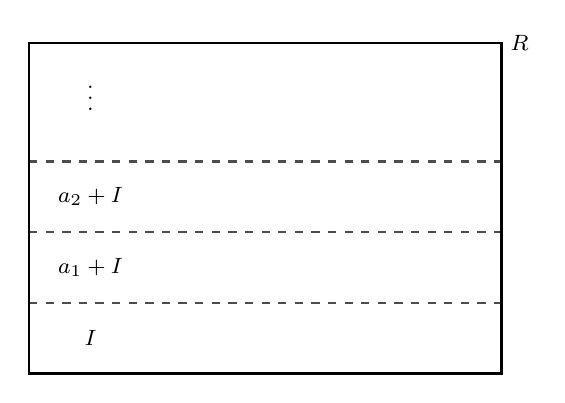
\begin{tikzpicture}[line width = 1,scale = 1.2]
\footnotesize
\draw[dashed, black!70] (0,0.75) -- (5,0.75);
\draw[dashed, black!70] (0,1.5) -- (5,1.5);
\draw[dashed, black!70] (0,2.25) -- (5,2.25);
\node[black] at (0.65,0.75/2) {$I$};
\node[black] at (0.65,{0.75+0.75/2}) {${a_1 + I}$};
\node[black] at (0.65,{1.5+0.75/2}) {${a_2 + I}$};
\node[black] at (0.65,{3}) {$\vdots$};
\node[anchor = west] at (5,3.5) {$R$};
\draw (0,0)--(5,0)--(5,3.5)--(0,3.5)--cycle;
\end{tikzpicture}
\end{center}

\begin{fact}\label{fact.AdditiveSubgroupRingQuotientProperties}
Let $I$ be an additive subgroup of a ring $R$. Then for all $a,b\in R$
\begin{enumerate}
\item $a + I = b+I$ if and only if $a-b\in I$ if and only if $a \in b + I$; and
\item either $(a + I )\cap (b+I )= \emptyset$ or $a + I = b + I$.
\end{enumerate}
\end{fact}

The goal is to understand when $R/I$ can be given the structure of a ring. To do this, we need to decide how to add and multiply cosets. We would like to define $(a + I) + (b + I) = (a+b) + I$ and $(a + I)(b + I) = ab + I$, but the worry is that these operations are not well-defined. That is, the coset $a + I$ goes by many names (since $a+I = a'+I$ for every $a' \in a+I$), so we have to make sure that our definitions for the operations do not depend on which names we use for the cosets. 

Now, as mentioned before, $I$ is a \emph{normal} subgroup of $(R,+)$, so we know that coset addition is well-defined. Let's see what we need for multiplication. 
Fix two arbitrary cosets $a + I$ and $b+I$. Then, for all $x,y\in I$, $a + I = (a+x)+I$ and $b+I = (b+y)+I$.
Thus, in order for coset multiplication to be well-defined, we need to ensure that \[ab + I = (a+x)(b+y)+I \text{ for all $a,b\in R$ and all $x,y\in I$}.\]
The desired picture is as follows.
\begin{center}
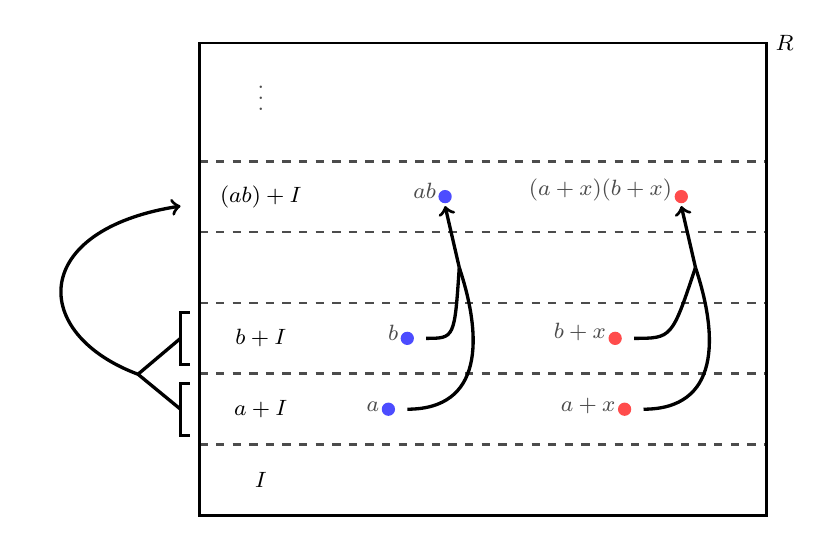
\begin{tikzpicture}[line width = 1, scale = 1.2]
\footnotesize
\draw[dashed, black!70] (0,0.75) -- (6,0.75);
\draw[dashed, black!70] (0,1.5) -- (6,1.5);
\draw[dashed, black!70] (0,2.25) -- (6,2.25);
\draw[dashed, black!70] (0,3) -- (6,3);
\draw[dashed, black!70] (0,3.75) -- (6,3.75);
\node[black] at (0.65,0.75/2) {$I$};
\node[black] at (0.65,{0.75+0.75/2}) {${a + I}$};
\node[black] at (0.65,{1.5+0.75/2}) {${b + I}$};
%\node[black!70] at (0.5,{2.25+0.75/2}) {\footnotesize$g_3N$};
\node[black] at (0.65,{3+0.75/2}) {${(ab)+I}$};
\node[black!70,anchor = -10] at (2,{0.75+0.75/2}) {$a$};\fill[blue!70] (2,{0.75+0.75/2}) circle (2pt);
\node[black!70,anchor = -20] at (2.2,{1.5+0.75/2}) {$b$};\fill[blue!70] (2.2,{1.5+0.75/2}) circle (2pt);
\node[black!70,anchor = -5] at (4.5,{0.75+0.75/2}) {$a+x$};\fill[red!70] (4.5,{0.75+0.75/2}) circle (2pt);
\node[black!70,anchor = -10] at (4.4,{1.5+0.75/2}) {$b+x$};\fill[red!70] (4.4,{1.5+0.75/2}) circle (2pt);
\node[black!70,anchor = -15] at (2.6,{3+0.75/2})  {$ab$};\fill[blue!70] (2.6,{3+0.75/2}) circle (2pt);
\node[black!70,anchor = -5] at (5.1,{3+0.75/2})  {$(a+x)(b+x)$};\fill[red!70] (5.1,{3+0.75/2}) circle (2pt);
\draw[black, line width = 1.2] (2.2,{0.75+0.75/2}) .. controls (3,{0.75+0.75/2} ) and (3,{1.5+0.75/2} ).. (2.75,{2.25+0.75/2});
\draw[black, line width = 1.2] (2.4,{1.5+0.75/2}) .. controls (2.7,{1.5+0.75/2} ).. (2.75,{2.25+0.75/2});
\draw[black, line width = 1.2,->] (2.75,{2.25+0.75/2}) -- (2.6,{3+0.75/2-0.1});
\draw[black,line width = 1.2] (4.7,{0.75+0.75/2}) .. controls (5.5,{0.75+0.75/2} ) and (5.5,{1.5+0.75/2} ).. (5.25,{2.25+0.75/2});
\draw[black,line width = 1.2] (4.6,{1.5+0.75/2}) .. controls (5,{1.5+0.75/2} ).. (5.25,{2.25+0.75/2});
\draw[black, line width = 1.2,->] (5.25,{2.25+0.75/2}) -- (5.1,{3+0.75/2-0.1});

\draw[black, line width = 1.2] (-0.1,{0.75+0.65}) -- (-0.2,{0.75+0.65}) -- (-0.2,{0.75+0.1})-- (-0.1,{0.75+0.1});
\draw[black, line width = 1.2] (-0.1,{1.5+0.65}) -- (-0.2,{1.5+0.65}) -- (-0.2,{1.5+0.1})-- (-0.1,{1.5+0.1});
\draw[black, line width = 1.2] (-0.2,{0.75+0.75/2}) -- (-0.65,{1.12+0.75/2});
\draw[black, line width = 1.2] (-0.2,{1.5+0.75/2}) -- (-0.65,{1.12+0.75/2});
\draw[black, line width = 1.2,->] (-0.65,{1.12+0.75/2}) .. controls (-1.8,{1.65+0.75/2-0.1}) and  (-1.8,{2.75+0.75/2-0.1}) .. (-0.2,{3+0.75/2-0.1});
\node[black!70] at (0.65,{4.5}) {$\vdots$};
\node[anchor = west] at (6,5) {$R$};
\draw (0,0)--(6,0)--(6,5)--(0,5)--cycle;
\end{tikzpicture}
\end{center} 
After distributing, we have $ab + I = ab + ay + xb + xy +I$, which simplifies to $I = ay + xb + xy +I$. By Fact~\ref{fact.AdditiveSubgroupRingQuotientProperties}, we see that what we really need to ensure is that 
\[ay + xb + xy\in I \text{ for all $a,b\in R$ and all $x,y\in I$}.\] 
In particular, this has to be true when $a=b=0$, which implies that $xy\in I$ for all $x,y\in I$, so $I$ needs to be closed under multiplication, hence a subring. So, let's assume that $I$ is a subring. Then, since $xy \in I$,  $ay + xb + xy\in I$ reduces to $ay + xb\in I$. So, assuming that $I$ is a subring, our previous condition becomes
\[ay + xb\in I \text{ for all $a,b\in R$ and all $x,y\in I$}.\] 
Now, if $a$ is arbitrary and $b=0$, then we see that $ay \in I$ for all $a\in R$ and $y\in I$. Similarly, we find that $xb \in I$ for all $b\in R$ and $x\in I$. These are new properties. In words, $I$ must be closed under (left and right) multiplication by elements from $R$. 

In conclusion, if $I$ is a subring that is closed under multiplication by elements from $R$ then the above addition and multiplication for $R/I$ is well-defined, making $R/I$ a ring. The converse is also true. As such, we give these special subrings a special name.

\begin{definition}
Let $R$ be a ring, and let $I\subseteq R$. Then $I$ is an \textbf{ideal} of $R$ if  
\begin{enumerate}
\item $I$ is a subring; and 
\item for all $r\in R$ and all $a\in I$, both $ra\in I$ and $ar\in I$.
\end{enumerate}
\end{definition}

Let's also summarize our work above about defining operations on the quotient $R/I$.

\begin{fact}\label{fact.QuotientRing}
Let $R$ be a ring and let $I$ be an ideal of $R$.  Then $R/I$ is a ring under the binary operations defined as follows. For all $a,b\in R$, 
\begin{itemize}
\item $(a+I)+(b+I)  =  (a+b)+I$;
\item $(a+I)(b+I)  = (ab)+I.$
\end{itemize}
\end{fact}

\begin{problem} For each subset of the given ring, determine if the subset is an ideal, a subring, or neither.
\begin{flushleft}
\tabulinesep = 1.8mm
\begin{tabu}  {X[2,r,m]|[2pt]X[c,m]|X[c,m]|X[c,m]}
 & ideal & subring & neither  \\ \tabucline[2pt]{-}
$\mathbb{Z}\subset \mathbb{Q}$ &&& \\  \hline 
$2\mathbb{Z}\subset \mathbb{Z}$  &&& \\ \hline 
$\{\text{odd integers}\}\subset \mathbb{Z}$  &&& \\ \hline 
$\{0,3,6,9\}\subset \mathbb{Z}_{12}$  &&& \\ \hline 
$\{p(x)\mid p(0)=0\}\subset \mathbb{Q}[x]$  &&& \\ \hline 
$\{\text{constant polynomials}\}\subset \mathbb{Q}[x]$  &&& \\ \hline 
\end{tabu}
\end{flushleft}
\end{problem}

\begin{problem}
Let $I = \{(x^2+1)p(x)\mid p(x) \in \mathbb{Q}[x]\}$. 
\begin{enumerate}
\item Show that $I$ is an ideal of $\mathbb{Q}[x]$.
\item Write out $5$ elements of $I$, each with a different degree.
\item Explain why $I$ contains polynomials of every degree larger than or equal to $2$.
\item Let $a(x) = x^4+3x+5$. Write out $5$ elements of the coset $a(x) + I$.
\item Find some $b(x)$ in the coset $a(x) + I$ such that $\deg b(x) = 1$.
\item Explain why $(x + I)^2 = -1 + I$ in the ring $\mathbb{Q}[x]/I$.
\end{enumerate}
\end{problem}

\begin{problem}\label{prob.RepresentPolyIdealsWithSmallDegree}
Let $I = \{(x^2+1)p(x)\mid p(x) \in \mathbb{Q}[x]\}$. Show that every coset $a(x) + I\in\mathbb{Q}[x]/I$ can be represented as $a(x) + I = r(x) + I$ for some $r(x) \in \mathbb{Q}[x]$ where  $\deg r(x) < 2$ or $r(x) = 0$.
\end{problem}

\begin{problem}\label{prob.RepresentIntegerIdealsWithSmallNumber}
Recall that $6\mathbb{Z} = \{6z \mid z\in \mathbb{Z}\}$.
\begin{enumerate}
\item Show that $6\mathbb{Z}$ is an ideal of $\mathbb{Z}$.
\item Show that $a + I = b + I$ if and only if $a \equiv_6 b$.
\item Show that for all $a + I\in\mathbb{Z}/6\mathbb{Z}$, $a + I = r + I$ for some $r \in \mathbb{Z}$ with $0 \le r < 6$.
%\item What familiar ring does $\mathbb{Z}/6\mathbb{Z}$ remind you of?
\end{enumerate}
\end{problem}

\begin{problem}
Let $I = \{3q \mid q\in \mathbb{Q}\}$.
\begin{enumerate}
\item Show that $I$ is an ideal of $\mathbb{Q}$.
\item Show that $1\in I$, and use this to explain why $I =  \mathbb{Q}$.
\end{enumerate}
\end{problem}

Let's record some observations from the previous problems.

\begin{theorem}\label{thm.MultiplesFormIdeal}
Let $R$ be a commutative ring, and let $a\in R$. The set $I = \{ar\mid r\in R\}$ is an ideal of $R$.
\end{theorem}

In the previous theorem, the set $\{ar\mid r\in R\}$ should be thought of as the set of all multiples of $a$, and it is often denoted $aR$ (as in $2\mathbb{Z}$).

\begin{theorem}\label{thm.IdealContainingUnitsEqualsR}
Assume $R$ is a ring with unity. Let $I$ be an ideal of $R$. If $I$ contains a unit of $R$, then $I = R$.
\end{theorem}

\begin{theorem}
Let $R$ be a ring. Then $\{0\}$ and $R$ are ideals of $R$.
\end{theorem}

\begin{theorem}\label{thm.CharacterizeFieldWithIdeals}
Assume $R$ is a commutative ring with $1\neq 0$. Then $R$ is a field if and only if the only ideals of $R$ are $\{0\}$ and $R$.
\end{theorem}

\begin{theorem}\label{thm.CommutativityPassestoQuotients}
Let $I$ be an ideal of a ring $R$.
\begin{enumerate}
\item If $R$ is a commutative ring, then $R/I$ is commutative ring.
\item If $R$ is a ring with unity, then $R/I$ is a ring with unity.
\end{enumerate}
\end{theorem}

% % % % % % % % % % % % % % % % % % % % % % % % % % % % % % % % % % % % % % % % % % % %
% SUBSECTION
% % % % % % % % % % % % % % % % % % % % % % % % % % % % % % % % % % % % % % % % % % % %
\subsection{Generating ideals}

As with groups and fields, we will want to generate subobjects from subsets. Generating ideals will be more useful for us that subrings, so we will only focus on ideals. Regarding notation, it is common to use $(A)$ for the ideal generated by $A$ instead of $\langle A \rangle$, and we will follow that convention. We begin with intersections.

\begin{theorem}
If $I$ and $J$ are ideals of a ring $R$, then $I\cap J$ is an ideal of $R$.
\end{theorem}

This can be generalized to arbitrary intersections. 

\begin{theorem}
If $\mathcal{C}$ is any collection of ideals of a ring $R$, then the intersection of all ideals from $\mathcal{C}$ is again an ideal of $R$.
\end{theorem}

Now, if $A$ is any subset of $R$, we can let $\mathcal{C}$ be the collection of all ideals containing $A$, to see that the intersection of all ideals containing $A$ is an ideal, and it must be the smallest ideal containing $A$. This leads to the following definition. 

\begin{definition}
Suppose $A$ is a subset of a ring $R$. The \textbf{ideal of $R$ generated by $A$}, denoted $(A)$, is defined to be the intersection of all ideals containing $A$.   An ideal generated by one element is a \textbf{principal ideal}. If $A = \{a_1,\ldots a_k\}$, we often write $(a_1,\ldots a_k)$ in place of $(A)$.
\end{definition}

\begin{problem}
Consider the ring $\mathbb{Z}$. 
\begin{enumerate}
\item Recall that $2\mathbb{Z}$ is an ideal of $\mathbb{Z}$. Now use the definition of $(2)$ to explain why $(2) \subseteq 2\mathbb{Z}$.
\item Use  that $(2)$ is an ideal containing $2$ to explain why $2\mathbb{Z}\subseteq (2)$. Conclude that $(2) = 2\mathbb{Z}$.
\item Use  that $(6,10)$ is an ideal containing $6$ and $10$, to write down 5 elements of $(6,10)$. 
\item Use the definition of $(6,10)$ to explain why $(6,10)\subseteq (2)$.
\item Use B\'ezout's lemma (Fact~\ref{Fact.Bezout}) to show that $(2) \subseteq (6,10)$. Conclude that $(6,10) = (2)$.
\item For arbitrary $m,n\in \mathbb{Z}$, do you think $(m,n) = (a)$ for some $a\in \mathbb{Z}$? Why or why not?
\end{enumerate}
\end{problem}

Let's work to abstract some of what we discovered in this problem.

\begin{theorem}\label{thm.PrincipalIdeals}
If $R$ is a commutative ring with unity, then $(a)=\{ar\mid r\in R\}$.
\end{theorem}

Theorem~\ref{thm.PrincipalIdeals} says that $(a)$ is precisely the set of all multiples of $a$. Or, in other words, $(a)$ is the set of all elements that are divisible by $a$. In particular, $(n) = n\mathbb{Z}$ in the ring $\mathbb{Z}$. But what about $(m,n)$?

\begin{theorem}
If $m,n\in \mathbb{Z}$ are nonzero, then $(m,n) = (d)$ where $d = \gcd(m,n)$.
\end{theorem}

In words, an ideal of $\mathbb{Z}$ that is generated by two elements can actually be generated by a single element. But more is true. The method for constructing the greatest common divisor for two elements can be easily adapted to show that \emph{any} ideal of $\mathbb{Z}$ can be generated by a single element, which yields the following fact.

\begin{fact}\label{fact.ZPID}
If $I$ is any ideal of $\mathbb{Z}$, then $I$ is a principle ideal. Moreover, if $I$ is not the zero ideal, then $I = (d)$ if and only if $d$ has the smallest possible absolute value among all nonzero elements of $I$.
\end{fact}

In fact, a similar result holds in any ring with a division algorithm. Importantly for us, this applies to polynomial rings over fields. Let's prove the result for ideals generated by two elements and leave the general case as a fact.

\begin{theorem}\label{thm.TwoGeneratedIsPrincipalFx}
Let $F$ be a field. If $a(x),b(x)\in F[x]$ are nonzero, then $(a(x),b(x)) = (d(x))$ where $d(x) = \gcd(a(x),b(x))$.
\end{theorem}

\begin{fact}\label{fact.FxPID}
Let $F$ be a field. If $I$ is any ideal of $F[x]$, then $I$ is a principle ideal. Moreover, if $I$ is not the zero ideal, then $I = (d(x))$ if and only if $d(x)$ has the smallest possible degree among all nonzero elements of $I$.
\end{fact}

\begin{problem}\label{prob.ShowIdealIsPrincipalQx}
Consider $a(x) = -x^2 -3x + 10$, $b(x) = 2x^2 + 8x - 10$, and $c(x) = x^3 - 2$ in $\mathbb{Q}[x]$.
\begin{enumerate}
\item Find a $d(x) \in \mathbb{Q}[x]$ such that $(a(x),b(x)) = (d(x))$. Is $(a(x),b(x)) = \mathbb{Q}[x]$? Explain.
\item Find a $d'(x) \in \mathbb{Q}[x]$ such that $(a(x),c(x)) = (d'(x))$. Is $(a(x),c(x)) = \mathbb{Q}[x]$? Explain.
\end{enumerate}
\end{problem}

We saw that $\mathbb{Z}$ and $F[x]$ have a special property: every ideal is a principal ideal. This does not happen in every ring, as we'll see, so rings with this property get a special name.

\begin{definition}
An integral domain is called a \textbf{principal ideal domain (PID)} if every ideal is a principal ideal.
\end{definition}

Thus, $\mathbb{Z}$ and $F[x]$ (for $F$ a field) are examples of PIDs. Let's show that $\mathbb{Z}[x]$ is not.

\begin{problem}
Consider the set $I:= \left\{2f(x) + xg(x)\mid f(x),g(x) \in \mathbb{Z}[x]\right\}$ in the ring $\mathbb{Z}[x]$. The set $I$ is an ideal of $\mathbb{Z}[x]$; you do \emph{not} need to prove this. Let's show that $I$ is not principal. Towards a contradiction, assume that $I = (d(x))$ for some $d(x)\in \mathbb{Z}[x]$.
\begin{enumerate}
\item Use the fact that $2\in I = (d(x))$ to show that $d(x)$ is a constant polynomial and, moreover, that $d(x) = \pm 1,\pm2$. 
\item Explain why every polynomial in $I$ has a constant term that is even, and use this to show that in fact $d(x) = \pm2$.
\item Now, we also know that $x\in I = (d(x))$. Why is this a contradiction?
\end{enumerate}
\end{problem}

Let's return to $\mathbb{Z}$, and put together what we have learned about its ideals. First, by Fact~\ref{fact.ZPID}, every ideal of $\mathbb{Z}$ is a principal ideal, so every ideal of $\mathbb{Z}$ is of the form $(n)$ for some $n\in \mathbb{Z}$. Moreover, Theorem~\ref{thm.PrincipalIdeals} tell us that $(n)$ is just the set of all multiple of $n$, so $(n) = n\mathbb{Z}$. Thus, we know all of the ideals of $\mathbb{Z}$, and we know that they have a nice form. But how do they fit together? Let's explore this.

\begin{theorem}\label{thm.IdealContainment}
Let $R$ be a commutative ring with unity, and let $a,b \in R$. Then $(a) \subseteq (b)$ if and only if $b$ divides $a$.
\end{theorem}

This theorem can be used to quickly draw portions of the lattice of ideals of $\mathbb{Z}$. For example, suppose we want to draw all of the ideals that contain the ideal $(45)$. Every ideal is principal; suppose $(n)$ is an ideal containing $(45)$. By Theorem~\ref{thm.IdealContainment}, $n$ must divide $45$. So, looking at all divisors of $45$ (and noticing that $(-n) = (n)$), we get the following lattice. 
\begin{center}
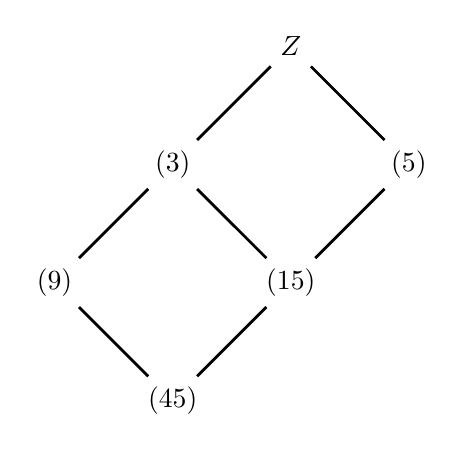
\begin{tikzpicture}[line width = 1, scale = 1.5]
\node (E) at (1,0) {$\mathbb{Z}$};
\node (F3) at (2,-1)  {$(5)$};
\node (F1F2) at (0,-1)  {$(3)$};
\node (F1) at (-1,-2) {$(9)$};
\node (F2) at (1,-2) {$(15)$};
\node (F1capF2) at (0,-3) {$(45)$};
\draw (E) -- (F1F2);\draw (E) -- (F3);
\draw (F1F2) -- (F1);\draw (F1F2) -- (F2);\draw (F3) -- (F2);
\draw (F1capF2) -- (F1);\draw (F1capF2) -- (F2);
\end{tikzpicture}
\end{center}

\begin{problem}
Draw the the lattice of ideals of $\mathbb{Z}$ that contain the ideal $(60)$.
\end{problem}

Let's focus on the ideals of $\mathbb{Z}$ that are at the top of the lattice but below $\mathbb{Z}$.

\begin{definition}
An ideal $M$ of a ring $R$ is called a \textbf{maximal ideal} if $M\neq R$ and the only ideals containing $M$ are $M$ and $R$.
\end{definition}

\begin{theorem}
An ideal $I$ of $\mathbb{Z}$ is maximal if and only if $I=(p)$ for some prime $p\in \mathbb{Z}$.
\end{theorem}

Since $F[x]$ (for $F$ a field) is also PID, it's relatively easy to study the ideals of $F[x]$ too. As with $\mathbb{Z}$, every ideal is a principal ideal, and we can use Theorem~\ref{thm.IdealContainment} to see how they fit together. There is one preliminary result that will help us avoid redundancies.

\begin{theorem}\label{thm.DifferByUnitSameIdeal}
Let $R$ be a commutative ring with unity. If $a \in R$ and $u\in U(R)$, then $(a) = (ua)$.
\end{theorem}

Now, suppose we want to find all of the ideals of $\mathbb{Q}[x]$ that contain the ideal $(x^2+5x+6)$. As before, Theorem~\ref{thm.IdealContainment} tells us that we should look at divisors of $x^2+5x+6$ in $\mathbb{Q}[x]$. Noting that $x^2+5x+6 =  (x+2)(x+3)$, we get the following. 
\begin{center}
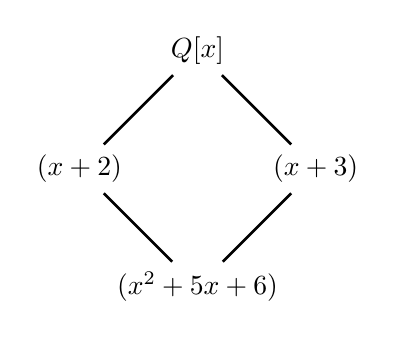
\begin{tikzpicture}[line width = 1, scale = 1.5]
\node (F1F2) at (0,-1)  {$\mathbb{Q}[x]$};
\node (F1) at (-1,-2) {$(x+2)$};
\node (F2) at (1,-2) {$(x+3)$};
\node (F1capF2) at (0,-3) {$(x^2+5x+6)$};
\draw (F1F2) -- (F1);\draw (F1F2) -- (F2);
\draw (F1capF2) -- (F1);\draw (F1capF2) -- (F2);
\end{tikzpicture}
\end{center}


\begin{problem}
Draw the the lattice of ideals of $\mathbb{Q}[x]$ that contain the ideal $(x^4 +x^2)$.
\end{problem}

\begin{theorem}\label{thm.MaximalIFFIrreducibleinFx}
Let $F$ be a field. An ideal $I$ of $F[x]$ is maximal if and only if $I=(p(x))$ for some irreducible polynomial $p(x)\in F[x]$.
\end{theorem}



% % % % % % % % % % % % % % % % % % % % % % % % % % % % % % % % % % % % % % % % % % % %
% % % % % % % % % % % % % % % % % % % % % % % % % % % % % % % % % % % % % % % % % % % %
% SECTION
% % % % % % % % % % % % % % % % % % % % % % % % % % % % % % % % % % % % % % % % % % % %
% % % % % % % % % % % % % % % % % % % % % % % % % % % % % % % % % % % % % % % % % % % %
\section{Homomorphisms}
As with groups, we use homomorphisms (and isomorphisms) to compare rings and fields.

\begin{definition}
Let $R$ and $S$ be rings. A map $\phi:R\to S$ is called a \textbf{ring homomorphism} if the following are true for all $a,b\in R$:
\begin{enumerate}
\item $\phi(a+b)=\phi(a)+\phi(b)$;
\item $\phi(ab)=\phi(a)\phi(b)$.
\end{enumerate}
If $\phi$ is a bijection, then $\phi$ is called an \textbf{isomorphism}, in which case, we say that $R$ and $S$ are \textbf{isomorphic rings} and write $R\cong S$.
\end{definition}

\begin{problem}\label{prob.HomomorphismCheckin}
Determine which of the following are ring homomorphisms. Explain.
\begin{enumerate}
\item $\phi: \mathbb{Z} \rightarrow 3\mathbb{Z}$ defined by $\phi(n) = 3n$
\item $\alpha: \mathbb{C} \rightarrow \mathbb{C}$ defined by $\alpha(a+bi) = a-bi$
\item $\beta: \mathbb{Z} \rightarrow \mathbb{Z}$ defined by $\beta(a) = a^3$
\item $f: \mathbb{Z}_3 \rightarrow \mathbb{Z}_3$ defined by $f(a) = a^3$
\item $g:  \mathbb{C}\rightarrow D_2\left(\mathbb{R}\right)$ defined by $\displaystyle g(a+bi) = \begin{bmatrix}a & 0 \\ 0 & b\end{bmatrix}$, where 
$\displaystyle D_2(\mathbb{R})=\left\{\begin{bmatrix}x & 0\\ 0 & y\end{bmatrix}\mid x,y\in \mathbb{R}\right\}$
\item\label{prob.HomomorphismCheckin.EvaluatePoly} $h: \mathbb{Q}[x] \rightarrow \mathbb{C}$ defined by $h(p(x)) = p(0)$
\end{enumerate}
\end{problem}

\begin{problem}
Which of the homomorphisms in Problem~\ref{prob.HomomorphismCheckin} were isomorphisms?
\end{problem}

In Problem~\ref{prob.HomomorphismCheckin}\ref{prob.HomomorphismCheckin.EvaluatePoly}, we saw that ``evaluating at zero'' was a homomorphism from $\mathbb{Q}[x]$ to  $\mathbb{C}$. At its core, this fact simply rests on how we add and multiply polynomials and does not require us to evaluate specifically at zero. For example, if $f(x),g(x)\in R[x]$ (for a ring $R$) and $c\in R$, then writing out $f(x)=a_0+\cdots+a_mx^m$ and $g(x)=b_0+\cdots+b_mx^m$ (with some $a_i$ and $b_j$ possible zero), we can show that $(f+g)(c) = f(c) + g(c)$. The analogous statement holds for multiplication too. We'll add in the details in the next theorem to see that ``evaluating at $c$'' is a homomorphism (whether or not $c = 0$).

\begin{theorem}[Evaluation homomorphism]\label{thm.EvalHom}
Let $R$ be a ring, and let $c\in R$. Define a function $\mathcal{E}_c:R[x] \rightarrow R$ by the rule $\mathcal{E}_c(p(x)) = p(c)$. Then $\mathcal{E}_c$ is a homomorphism.
\end{theorem}

Let's prove some general properties about homomorphisms.

\begin{theorem}
Let $\phi:R\to S$  be a ring homomorphism. Then 
\begin{enumerate}
\item $\phi(0) = 0$; and
\item for all $a\in R$, $\phi(-a) = -\phi(a)$.
\end{enumerate}
\end{theorem}

\begin{theorem}
Suppose that $R$ is a ring with unity. Let $\phi:R\to S$  be a ring homomorphism.  Then 
\begin{enumerate}
\item $\phi(1) = 1$; and
\item for all $a\in U(R)$, $\phi(a^{-1}) = (\phi(a))^{-1}$.
\end{enumerate}
\end{theorem}

\begin{theorem}[Composition of homomorphisms]
Let $\phi:R_1\to R_2$ and $\psi:R_2\to R_3$ be ring homomorphisms. Then $\psi\circ\phi:R_1 \to R_3$ is also a ring homomorphism.
\end{theorem}

There are two  important sets attached to homomorphisms: the kernel and the image.

\begin{definition}
Let $\phi:R\to S$ be a ring homomorphism. 
\begin{itemize}
\item The \textbf{kernel} of $\phi$, denote $\ker \phi$, is $\ker \phi=\{a\in R\mid \phi(a)=0\}$. 
\item The \textbf{image} of $\phi$, denoted  $\operatorname{im}\phi$ or  $\phi(R)$, is $\operatorname{im}\phi=\{b\in S\mid b=\phi(a) \text{ for some $a\in R$}\}$.
\end{itemize}
\end{definition}

\begin{problem}\label{prob.KernelImageConcrete}
Determine the kernel and image of each homomorphism.
\begin{enumerate}
\item $\alpha: \mathbb{Q}[x] \rightarrow \mathbb{C}$ defined by $\alpha(p(x)) = p(0)$
\item $\beta: \mathbb{Z} \rightarrow \mathbb{Z}_5$ defined by $\beta(n) = n \text{ (mod $5$)}$
\end{enumerate}
\end{problem}

\begin{problem}\label{prob.NaturalProjection}
Let $I$ be an ideal of a ring $R$. Define a function $\pi:R \rightarrow R/I$ by $\pi(r) = r+I$.
\begin{enumerate}
\item Show that $\pi$ is a homomorphism. %(The map $\pi$ is often called the \textit{natural projection} of $R$ onto $R/I$.)
\item What is the kernel of $\pi$?
\item What is the image of $\pi$?
\end{enumerate}
\end{problem}

As with groups, the kernel and image of a homomorphism have special properties and can be used to detect if a function is injective (one-to-one) or surjective (onto).

\begin{theorem}\label{thm.KernelIsIdealImageIsSubring}
Let $\phi:R\to S$ be a ring homomorphism. Then $\ker(\phi)$ is an ideal of $R$, and $\operatorname{im}\phi$ is a subring of $S$.
\end{theorem}

\begin{theorem}\label{thm.HomInjectiveSurjective}
Let $\phi:R\to S$ be a ring homomorphism. Then
\begin{enumerate}
\item $\phi$ is injective if and only if $\ker \phi = \{0\}$, and 
\item $\phi$ is surjective if and only if $\operatorname{im}\phi = S$.
\end{enumerate}
\end{theorem}

\begin{problem}\label{prob.EvalAtI}
By Theorem~\ref{thm.EvalHom}, the ``evaluation at $i$'' function from $\mathbb{C}[x]$ to  $\mathbb{C}$ is a homomorphism.  We can restrict the domain to $\mathbb{Q}[x]$ to obtain a homomorphism from $\mathcal{E}_{i}:\mathbb{Q}[x]\rightarrow\mathbb{C}$ defined by $\mathcal{E}_{i}(p(x)) = p(i)$, where $i$ denotes the usual complex number.
\begin{enumerate}
\item Show that $x^2+1$ is in $\ker \mathcal{E}_{i}$.
\item By Fact~\ref{fact.FxPID}, $\ker \mathcal{E}_{i} = (m(x))$ for some $m(x)\in \mathbb{Q}[x]$. Use the fact that $x^2+1$ is irreducible in $\mathbb{Q}[x]$, to show that $m(x) = a(x^2+1)$ for some nonzero constant $a\in \mathbb{Q}$.
\item Explain why $\ker \mathcal{E}_{i} = (x^2 + 1)$ (where $(x^2 + 1)$ is the ideal generated by $x^2 + 1$).
\item Explain why all of $\mathbb{Q}$ as well as $i$ are contained in the image of $\mathcal{E}_{i}$.
\item Explain why the image of $\mathcal{E}_{i}$ is contained in $\mathbb{Q}(i)$.
\end{enumerate}
\end{problem}

% % % % % % % % % % % % % % % % % % % % % % % % % % % % % % % % % % % % % % % % % % % %
% SUBSECTION
% % % % % % % % % % % % % % % % % % % % % % % % % % % % % % % % % % % % % % % % % % % %
\subsection{First Isomorphism Theorem}

The proof of the First Isomorphism Theorem for rings is essentially the same as for groups. Suppose we have a ring homomorphism $\phi:R\to S$. In order for $\phi$ to be an isomorphism, it must also be one-to-one and onto, but it may very well not be. However, with some slight adjustments, we can modify it to be both one-to-one and onto.

First, to make $\phi$ surjective, we change the codomain from $S$ to $\phi(R)$, i.e.~the image of $\phi$. Technically, we have a different function now, but we will still call it $\phi$. Anyway, $\phi:R\to \phi(R)$ is now surjective (by the definition of the image). But how do we make it one-to-one? By Theorem~\ref{thm.HomInjectiveSurjective}, we need  the kernel to be trivial. To accomplish, we work in quotient ring $R/ \ker \phi$. This has the effect of  collapsing all elements in the kernel to a single element (the  coset $\ker \phi$) that maps to $0$. Setting $K:= \ker \phi$, the picture is like this.

\begin{center}
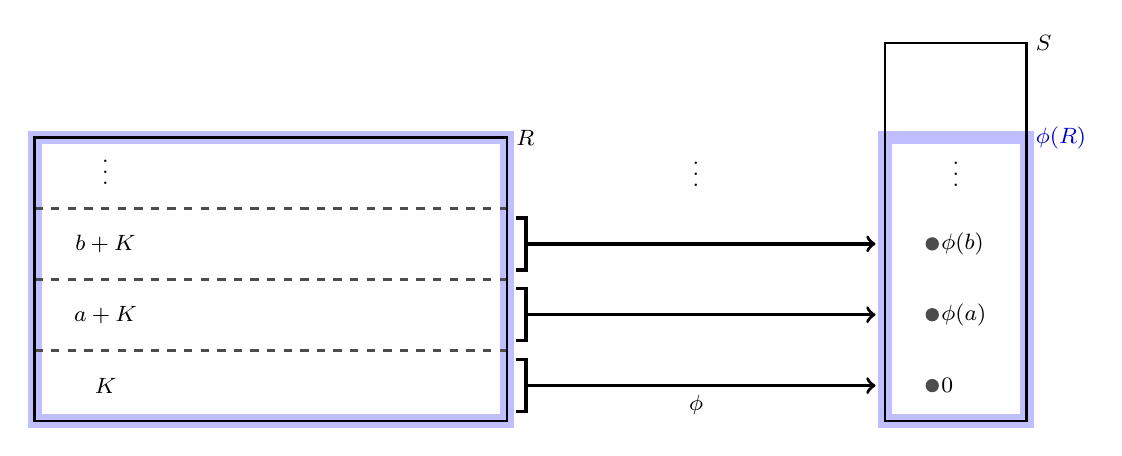
\begin{tikzpicture}[line width = 1, scale = 1.2]
\footnotesize
\draw[blue!25, line width = 5] (0,0)--(5,0)--(5,3)--(0,3)--cycle;
\foreach \i in {1,2,3} {
\draw[dashed, black!70] (0,\i*0.75) -- (5,\i*0.75);
\draw[black, line width = 1.2] (5.1,{(\i-1)*0.75+0.65}) -- (5.2,{(\i-1)*0.75+0.65}) -- (5.2,{(\i-1)*0.75+0.1})-- (5.1,{(\i-1)*0.75+0.1});
\draw[black, line width = 1.2,->] (5.2,{(\i-1)*0.75+0.75/2}) -- (8.9,{(\i-1)*0.75+0.75/2});
}
\node at (7,{3*0.75+0.45}) {$\vdots$};
\node[anchor = north] at (7,{0.75/2}) {$\phi$};
\node[black] at (0.75,0.75/2) {${ K}$};
\node[black] at (0.75,{0.75+0.75/2}) {${a + K}$};
\node[black] at (0.75,{1.5+0.75/2}) {${b+ K}$};
\node[black] at (0.75,{2.35+0.75/2}) {$\vdots$};
\node[anchor = west] at (5,3) {$R$};
\draw (0,0)--(5,0)--(5,3)--(0,3)--cycle;
\draw[black, line width = 1.2] (5.1,{0.75+0.65}) -- (5.2,{0.75+0.65}) -- (5.2,{0.75+0.1})-- (5.1,{0.75+0.1});
\begin{scope}[shift = {(9,0)}]
\draw[blue!25, line width = 5] (0,0)--(1.5,0)--(1.5,3)--(0,3)--cycle;
%\foreach \i in {1,2,...,5} {\draw[dashed, black!70] (0,\i*0.75) -- (1.5,\i*0.75);}
\foreach \i in {1,2,3} {\fill[black!70] (0.5,{(\i-1)*0.75+0.75/2}) circle (2pt);}
\node[anchor = west] at (0.5,{0.75/2}) {$0$};
\node[anchor = west] at (0.5,{0.75+0.75/2}) {$\phi(a)$};
\node[anchor = west] at (0.5,{2*0.75+0.75/2}) {$\phi(b)$};
\node[black] at (0.75,{3*0.75+.45}) {$\vdots$};
%\node[black] at (0.75,{5*0.75+0.75}) {$\boldsymbol\vdots$};
\node[anchor = west] at (1.5,4) {$S$};
\node[blue!80!black,anchor = west] at (1.5,3) {$\phi(R)$};
\draw (0,0)--(1.5,0)--(1.5,4)--(0,4)--cycle;
\end{scope}
\end{tikzpicture}
\end{center}

\begin{theorem}[First Isomorphism Theorem for Rings]\label{thm.FirstIsoRings}
If $\phi:R\to S$ is a ring homomorphism, then  $R/\ker \phi\cong \operatorname{im} \phi$.
\end{theorem}

\begin{problem}
Use the First Isomorphism Theorem together Problem~\ref{prob.KernelImageConcrete} to prove each of the following. 
\begin{enumerate}
\item $\mathbb{Q}[x]/(x) \cong \mathbb{Q}$ (where $(x)$ is the ideal generated by $x$)
\item $\mathbb{Z}/5\mathbb{Z} \cong \mathbb{Z}_5$
\end{enumerate}
\end{problem}

We now work towards a very nice and useable criterion to determine when a quotient ring is actually a field. Our approach will rely on Theorem~\ref{thm.CharacterizeFieldWithIdeals}, so we need to be able determine the relationship between ideals of $R$ and ideals of the quotient $R/I$. We will investigate this via homomorphisms, which we can then apply to $R/I$ using Problem~\ref{prob.NaturalProjection}.

\begin{theorem}\label{thm.Image}
Let $\phi:R\to S$ be a surjective ring homomorphism. If $I$ is an ideal of $R$, then $\phi(I)=\{b\in S\mid b=\phi(a) \text{ for some $a\in I$}\}$ (called the \textbf{image} of $I$) is an ideal of $S$.
\end{theorem}

\begin{theorem}\label{thm.InverseImage}
Let $\phi:R\to S$ be a ring homomorphism. If $J$ is an ideal of $S$, then $\phi^{-1}(J) := \{a\in R\mid\phi(a) \in J\}$ (called the \textbf{inverse image} of $J$) is an ideal of $R$ and, moreover,  $\ker\phi \subseteq \phi^{-1}(J)$.
\end{theorem}

Combining Theorems~\ref{thm.Image} and~\ref{thm.InverseImage} with Theorem~\ref{thm.CharacterizeFieldWithIdeals} yields the following result.

\begin{theorem}
Let $R$ be a commutative ring with $1\neq0$. Suppose $\phi:R\to S$ is a surjective ring homomorphism. Then $\ker\phi$ is maximal ideal of $R$ if and only if $S$ is field.
\end{theorem}

In light of Problem~\ref{prob.NaturalProjection}, our desired criterion for when a quotient ring is  a field is a relatively quick consequence of the previous result. 

\begin{theorem}\label{thm.QuotientIsField}
Let $R$ be a commutative ring with $1\neq0$. Then $I$ is maximal ideal of $R$ if and only if $R/I$ is field.
\end{theorem}

\begin{problem}\label{prob.EvalAtI-Take2}
Let's revisit Problem~\ref{prob.EvalAtI}.
\begin{enumerate}
\item Use Theorems~\ref{thm.MaximalIFFIrreducibleinFx} and~\ref{thm.QuotientIsField} to explain why $\mathbb{Q}[x]/(x^2+1)$ is a field.
\item Use Theorem~\ref{thm.FirstIsoRings} (and Problem~\ref{prob.EvalAtI}) to explain why the image of $\mathcal{E}_{i}:\mathbb{Q}[x]\rightarrow\mathbb{C}$ is a field that contains $\mathbb{Q}$ and $i$.
\item Explain why the image of $\mathcal{E}_{i}$ must be  $\mathbb{Q}(i)$, and conclude that $\mathbb{Q}[x]/(x^2+1) \cong \mathbb{Q}(i)$.
\end{enumerate}
\end{problem}

Let's end this section (as well as this decidedly long chapter!) by mentioning that there is an analog of Theorem~\ref{thm.QuotientIsField} characterizing when $R/I$ is an integral domain. The condition is that $I$ is a so-called \textit{prime} ideal. The result is tangential to our story, so we'll leave it for another time (see \href{https://en.wikipedia.org/wiki/Prime_ideal#Connection_to_maximality}{Wikipedia} or most any other book on abstract algebra).




